%!TEX root =  main.tex
%The sensors are differentiated in terms of their prediction efficiency and cost. 

\todoc[inline]{
On \cref{wrap-fig:1}:
Why is $Y_t$ the input of the first sensor?
	Should $Y_t$ appear on the figure at all?
	Should not each box take $Z_t$ as input?
	Also, perhaps it should be explained that $Z_t$ is not available
	to the learner. The dotted line should have an arrow at the end?
	}


\todoc[inline]{Starting with a specific example would be much better.}
A learner has access to $K\geq 2$ sensors that provide predictions
of an unknown label. It is assumed that the sensors form a cascade,
i.e., they are  \emph{ordered} in terms of their prediction efficiency,
later sensors are more accurate in predicting the unknown label.
However, acquiring the output of later sensors comes at a fixed cost.
The dilemma of the learner is that while he knows the ordering of the sensors,
the accuracies of the sensors are unknown.
The learner's task is to minimize the total prediction cost, which includes
both the cost of acquiring the sensor outputs and the cost incurred due to imperfect
sensor output.
The learner knows the costs, but does not know how efficient the sensors are
and learns only the output of the sensors.
Learning happens in a sequential setting, where in each round the learner can decide
sequentially (within the round) which sensor outputs to observe,
while respecting the ordering of the sensors.
The output of the last sensor selected serves as the prediction for the round.
\todoc{It is not evident why not combine the output of the sensors.}

Let $\{Z_t, Y_t\}_{{t>0}}$ denote a sequence generated according to an unknown distribution. $Z_t \in\mathcal{C} \subset  \mathcal{R}^d$, where $\mathcal{C}$ is a compact set, denotes a feature vector/context at time $t$ and $Y_t \in \{0,1\}$ its binary label. We denote output/prediction of the $i^{th}$ sensor as $\hat{Y}^i_t$ when its input is $Z_t$. The set of actions available to the learner is $\mathcal{A}=\{1,\ldots, K\}$, where  the action $k \in \mathcal{A}$ indicates acquiring predictions from sensors $1,\ldots, k$ and classifying using the prediction $\hat{Y}^k_t$. 


\begin{wrapfigure}{r}{5cm}
	\vspace{-.5cm}
	\centering
	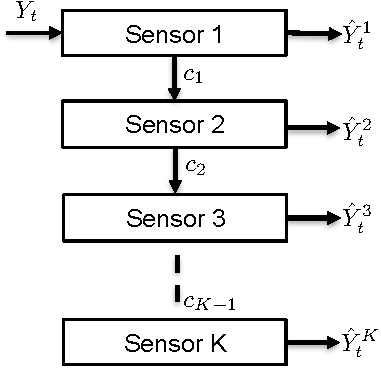
\includegraphics[scale=.6]{SensorCascade.pdf}
	\caption{Cascade of sensors
	}\label{wrap-fig:1}
	\vspace{-.5cm}
\end{wrapfigure} 



The prediction error rate of the $i^{th}$ sensor is denoted as $\gamma_i:=\Pr\{Y_t\neq \hat{Y}^k_t\}$. The learner incurs an extra cost of $c_k\geq 0$ to acquire output of sensor $k$ after acquiring output of sensor $k-1$. The sensor cascade is depicted in the adjacent figure. In this section we assume that the error rate does not depend on the  context, and the treatment with contextual information is given in the supplementary. 

Let $H_t(k)$ denote the feedback observed in round $t$ from action $k$. Since we observe predictions of all the first $k$ senors by playing action $k$, we get   $H_t(k)=(\hat{Y}^1_t,\ldots,\hat{Y}^k_t)$.
The loss incurred in each round is defined in terms of the prediction error and the total cost involved. When the learner selects action $k$, loss is the prediction error of sensor $k$ plus sum of the costs incurred along the path ($c_1,\ldots,c_k$). Let $L_t: \mathcal{A}\rightarrow \mathcal{R}_+$ denote the loss function in round $t$. Then,
\begin{equation}
L_t(k)=\mathbf{1}_{\{\hat{Y}^k_t\neq Y_t\}}+\sum_{j=1}^k c_j.
\end{equation} 
We refer to the above setup as Sensor Acquisition Problem (SAP) and denote it as $\psi=(K,\mathcal{A}, (\gamma_i,c_{i-1})_{i\in [K]})$\footnote{Note that $k\in \mathcal{A}$ implies that action $k$ selects all sensors ${1, 2, \cdots, k}$, not just sensor $k$. We set $c_0=0$}. A policy $\pi^\psi=(\pi^\psi_1, \pi^\psi_2, \cdots)$ on $\psi$, where  $\pi^\psi_t : \mathcal{H}_{t-1}\rightarrow
\mathcal{A}$, gives action selected in each round using history $\mathcal{H}_{t-1}$ that consists of all actions and corresponding feedback observed before $t$. Let $\Pi^\psi$ denote set of policies on $\psi$. For any $\pi \in \Pi^\psi$, we compare its performance with respect to the optimal policy (single best action in hindsight) and define its expected regret as follows
\begin{equation}
R^\psi_T(\pi)= \mathbb{E}\left[\sum_{t=1}^T L_t(a_t)\right]-\min_{k\in A}\mathbb{E}\left[\sum_{t=1}^T L_t(k)\right],
\end{equation}
where $a_t$ denotes the policy selected by $\pi_t$ in round $t$.
The goal of the learner is to learn a policy that minimizes the expected total loss, or, equivalently, to minimize the expected regret, i.e.,
\begin{equation}
\pi^*= \arg \min_{\pi \in \Pi^\psi } R^\psi_T(\pi).
\end{equation}

\noindent
{\bf Optimal action in hindsight: } For any $t$, we have 
\begin{equation}
\label{eqn:OptimalAction}
\mathbb{E}[L_t(k)]=\Pr\{Y_t\neq \hat{Y}^k_t\}+\sum_{j=1}^kc_j=\gamma_k +\sum_{j=1}^kc_j.
\end{equation}
Let $k^*=\arg\min_{k\in \mathcal{A}} \gamma_k + \sum_{i< k}c_i$. Then the optimal policy is to play action $k^*$ in each round. If an action $i$ is played in any round then it adds   $\Delta_k:=\gamma_k + \sum_{i<k}c_i -( \gamma_{k^*} + \sum_{i<k^*}c_i)$ to the expected regret. Let $I_t$ denote the action selected in round $t$ and $N^\psi_k(s)$ denote the number of times action $k$ is selected till time $s$, i.e., $N^\psi_k(s)=\sum_{t=1}^s \boldsymbol{1}_{\{I_t=k\}}$. Then the expected regret can be expressed as
\begin{eqnarray}
\label{eqn:ExpRegretGap}
R^\psi_T(\pi)&=& \sum_{k \in \mathcal{A}}\mathbb{E}[N_k^\psi(T)]\Delta_k.
\end{eqnarray}\

